% Options for packages loaded elsewhere
\PassOptionsToPackage{unicode}{hyperref}
\PassOptionsToPackage{hyphens}{url}
\PassOptionsToPackage{dvipsnames,svgnames,x11names}{xcolor}
%
\documentclass[
  12pt,
]{article}

\usepackage{amsmath,amssymb}
\usepackage[]{crimson}
\usepackage{setspace}
\usepackage{iftex}
\ifPDFTeX
  \usepackage[T1]{fontenc}
  \usepackage[utf8]{inputenc}
  \usepackage{textcomp} % provide euro and other symbols
\else % if luatex or xetex
  \usepackage{unicode-math}
  \defaultfontfeatures{Scale=MatchLowercase}
  \defaultfontfeatures[\rmfamily]{Ligatures=TeX,Scale=1}
\fi
% Use upquote if available, for straight quotes in verbatim environments
\IfFileExists{upquote.sty}{\usepackage{upquote}}{}
\IfFileExists{microtype.sty}{% use microtype if available
  \usepackage[]{microtype}
  \UseMicrotypeSet[protrusion]{basicmath} % disable protrusion for tt fonts
}{}
\usepackage{xcolor}
\usepackage[left = 1in, right = 1in, top = 1in, bottom =
1.5in]{geometry}
\setlength{\emergencystretch}{3em} % prevent overfull lines
\setcounter{secnumdepth}{5}
% Make \paragraph and \subparagraph free-standing
\ifx\paragraph\undefined\else
  \let\oldparagraph\paragraph
  \renewcommand{\paragraph}[1]{\oldparagraph{#1}\mbox{}}
\fi
\ifx\subparagraph\undefined\else
  \let\oldsubparagraph\subparagraph
  \renewcommand{\subparagraph}[1]{\oldsubparagraph{#1}\mbox{}}
\fi


\providecommand{\tightlist}{%
  \setlength{\itemsep}{0pt}\setlength{\parskip}{0pt}}\usepackage{longtable,booktabs,array}
\usepackage{calc} % for calculating minipage widths
% Correct order of tables after \paragraph or \subparagraph
\usepackage{etoolbox}
\makeatletter
\patchcmd\longtable{\par}{\if@noskipsec\mbox{}\fi\par}{}{}
\makeatother
% Allow footnotes in longtable head/foot
\IfFileExists{footnotehyper.sty}{\usepackage{footnotehyper}}{\usepackage{footnote}}
\makesavenoteenv{longtable}
\usepackage{graphicx}
\makeatletter
\def\maxwidth{\ifdim\Gin@nat@width>\linewidth\linewidth\else\Gin@nat@width\fi}
\def\maxheight{\ifdim\Gin@nat@height>\textheight\textheight\else\Gin@nat@height\fi}
\makeatother
% Scale images if necessary, so that they will not overflow the page
% margins by default, and it is still possible to overwrite the defaults
% using explicit options in \includegraphics[width, height, ...]{}
\setkeys{Gin}{width=\maxwidth,height=\maxheight,keepaspectratio}
% Set default figure placement to htbp
\makeatletter
\def\fps@figure{htbp}
\makeatother
\newlength{\cslhangindent}
\setlength{\cslhangindent}{1.5em}
\newlength{\csllabelwidth}
\setlength{\csllabelwidth}{3em}
\newlength{\cslentryspacingunit} % times entry-spacing
\setlength{\cslentryspacingunit}{\parskip}
\newenvironment{CSLReferences}[2] % #1 hanging-ident, #2 entry spacing
 {% don't indent paragraphs
  \setlength{\parindent}{0pt}
  % turn on hanging indent if param 1 is 1
  \ifodd #1
  \let\oldpar\par
  \def\par{\hangindent=\cslhangindent\oldpar}
  \fi
  % set entry spacing
  \setlength{\parskip}{#2\cslentryspacingunit}
 }%
 {}
\usepackage{calc}
\newcommand{\CSLBlock}[1]{#1\hfill\break}
\newcommand{\CSLLeftMargin}[1]{\parbox[t]{\csllabelwidth}{#1}}
\newcommand{\CSLRightInline}[1]{\parbox[t]{\linewidth - \csllabelwidth}{#1}\break}
\newcommand{\CSLIndent}[1]{\hspace{\cslhangindent}#1}

\usepackage{booktabs}
\usepackage{longtable}
\usepackage{array}
\usepackage{multirow}
\usepackage{wrapfig}
\usepackage{float}
\usepackage{colortbl}
\usepackage{pdflscape}
\usepackage{tabu}
\usepackage{threeparttable}
\usepackage{threeparttablex}
\usepackage[normalem]{ulem}
\usepackage{makecell}
\usepackage{xcolor}
\usepackage[scale = 0.75]{sourcecodepro}
\usepackage{etoolbox}
\usepackage{enumitem}
\setlist[description]{leftmargin=\parindent,labelindent=\parindent}
\makeatletter
\makeatother
\makeatletter
\makeatother
\makeatletter
\@ifpackageloaded{caption}{}{\usepackage{caption}}
\AtBeginDocument{%
\ifdefined\contentsname
  \renewcommand*\contentsname{Table of contents}
\else
  \newcommand\contentsname{Table of contents}
\fi
\ifdefined\listfigurename
  \renewcommand*\listfigurename{List of Figures}
\else
  \newcommand\listfigurename{List of Figures}
\fi
\ifdefined\listtablename
  \renewcommand*\listtablename{List of Tables}
\else
  \newcommand\listtablename{List of Tables}
\fi
\ifdefined\figurename
  \renewcommand*\figurename{Figure}
\else
  \newcommand\figurename{Figure}
\fi
\ifdefined\tablename
  \renewcommand*\tablename{Table}
\else
  \newcommand\tablename{Table}
\fi
}
\@ifpackageloaded{float}{}{\usepackage{float}}
\floatstyle{ruled}
\@ifundefined{c@chapter}{\newfloat{codelisting}{h}{lop}}{\newfloat{codelisting}{h}{lop}[chapter]}
\floatname{codelisting}{Listing}
\newcommand*\listoflistings{\listof{codelisting}{List of Listings}}
\makeatother
\makeatletter
\@ifpackageloaded{caption}{}{\usepackage{caption}}
\@ifpackageloaded{subcaption}{}{\usepackage{subcaption}}
\makeatother
\makeatletter
\@ifpackageloaded{tcolorbox}{}{\usepackage[many]{tcolorbox}}
\makeatother
\makeatletter
\@ifundefined{shadecolor}{\definecolor{shadecolor}{rgb}{.97, .97, .97}}
\makeatother
\makeatletter
\makeatother
\ifLuaTeX
  \usepackage{selnolig}  % disable illegal ligatures
\fi
\IfFileExists{bookmark.sty}{\usepackage{bookmark}}{\usepackage{hyperref}}
\IfFileExists{xurl.sty}{\usepackage{xurl}}{} % add URL line breaks if available
\urlstyle{same} % disable monospaced font for URLs
\hypersetup{
  pdftitle={Shades of Blue: Racial Imagery of Police and White Attitudes toward Policing},
  pdfauthor={Chaoyue Wang},
  colorlinks=true,
  linkcolor={NavyBlue},
  filecolor={Maroon},
  citecolor={NavyBlue},
  urlcolor={Cyan4},
  pdfcreator={LaTeX via pandoc}}

\title{\textbf{Shades of Blue: Racial Imagery of Police and 
White Attitudes toward Policing}}

\date{December 6, 2022}

\begin{document}
\urlstyle{tt}

\maketitle

%----------------------------------------------
%   Abstract
%----------------------------------------------

\thispagestyle{empty}

\begin{abstract} 
\noindent %\onehalfspacing 
Following the murder of George Floyd, whites and blacks again diverged
in their perceptions of and reactions to the reality of police violence
in the United States. Compared to people of color, white Americans are
more supportive of police agencies and more hesitant about reforming
policing behavior even in the wake of multiple recent police-involved
fatla shootings. While existing works look into experiential and
cultural differences between the two groups, this study examines the
role of whites' excessive representation in police workforce that
fosters a ``white imagery'' of the profession. Can this racialized image
of police officers activate in-group favoritism among whites but push
blacks away? Merging the 2020 Cooperative Election Study with
administrative sampling of local police departments, I find that given
whites' share of local population constant, a higher percentage of white
officers in local police department is associated with more favorable
feelings of police among whites, and a greater black-white divide in
police attitudes. In the presence of police violence, a whiter police
workforce also makes white residents more tolerant of police officers.
\end{abstract}

\begin{center}
	\textbf{Word Count: 6,073}
\end{center} 

\begin{quote}
%\textbf{Keywords}: Keywords go here. \\
% \noindent \textbf{Note}: Note on replication data.
\end{quote}

%================Begin Manuscript==================
\newpage \clearpage \pagenumbering{arabic}\captionsetup{labelfont = bf, font = small}

\AtBeginEnvironment{tabular}{\small}

\AtBeginEnvironment{tablenotes}{\small}

\urlstyle{tt}

\ifdefined\Shaded\renewenvironment{Shaded}{\begin{tcolorbox}[sharp corners, breakable, enhanced, interior hidden, boxrule=0pt, borderline west={3pt}{0pt}{shadecolor}, frame hidden]}{\end{tcolorbox}}\fi

\setstretch{1.5}
\hypertarget{introduction}{%
\section{Introduction}\label{introduction}}

On May 25 of 2020, George Floyd, an unarmed 46-year-old African American
man, was choked to death in Minneapolis, Minnesota while a white local
police officer knelt on his neck for over nine minutes. This blatant
instance of political brutality, along with multiple police-involved
homicides under intense public scrutiny, brings about a national debate
on how police and policing behavior should be constrained. Similar to
many other issues in American politics, a racial cleavage emerges in the
public's response to police violence. Compared to people of color,
especially African Americans, whites are in general more approving of
police performance, and more likely to regard fatal encounters with
police as isolated incidents rather than indications of larger problems
(\protect\hyperlink{ref-desilver}{Desilver, Lipka, and Fahmy 2020};
\protect\hyperlink{ref-morin2016}{Morin and Stepler 2016}). In terms of
proactive moves to address police brutality, whites are also less likely
to support the Black Lives Matter movement or defunding the police to
better finance other public programs
(\protect\hyperlink{ref-thomas}{Thomas and Horowitz 2020}). Behind this
attitudinal gap on police is an extensive division between whites and
blacks regarding their perception of the criminal justice system
(\protect\hyperlink{ref-hurwitz2005}{Hurwitz and Peffley 2005};
\protect\hyperlink{ref-peffley2010}{Peffley and Hurwitz 2010};
\protect\hyperlink{ref-sigelman1997}{Sigelman et al. 1997}).

Why do people of distinct racial identities come to divergent responses
to the same institution? Some studies have emphasized the role of lived
experiences of blacks and whites, with the former far more intensely
scrutinized and confronted by law enforcement agencies during their life
course (\protect\hyperlink{ref-alvarado2020}{Alvarado 2020};
\protect\hyperlink{ref-peffley2010}{Peffley and Hurwitz 2010}). Prior
information and expectations established from these experiences set
apart the ways black and white citizens process events of police
violence (\protect\hyperlink{ref-jefferson2021}{Jefferson, Neuner, and
Pasek 2021}). Attention is also called to the possibility that cultural
or social processes can drive blacks and whites to different conclusions
even in the face of similar information. For example, racial differences
in attribution between structure versus agency may matter: whereas
blacks tend to see police violence as product of institutional ills,
whites are more likely to blame the persons killed for their
wrongdoings, leaving views on police intact
(\protect\hyperlink{ref-israel-trummel2022}{Israel-Trummel and Streeter
2022}; \protect\hyperlink{ref-streeter2019}{Streeter 2019}).

Jefferson, Neuner, and Pasek
(\protect\hyperlink{ref-jefferson2021}{2021}) focus on how the incidents
of police violence are themselves racialized in the public mind: indeed,
all cases of fatal police encounters that received intense scrutiny from
the public in 2020, like that of Jacob Blake and George Floyd, involve a
black victim and a white officer. With these racial images in mind,
whites and blacks engage in ``race-based motivated reasoning'',
predisposed to blame black victims and white officers respectively as
``an emotional or affective commitment'' to defending their racial
in-groups (\protect\hyperlink{ref-jefferson2021}{Jefferson, Neuner, and
Pasek 2021, 1166}). In this sense, the racial gap in perceiving police
exemplify the imbalance of racial dynamics within the practice of
policing itself. Whites' imagination of blacks as criminal and violent
is well documented, and is shown to affect whites' preferences on law
enforcement (\protect\hyperlink{ref-hurwitz1997}{Hurwitz and Peffley
1997}; \protect\hyperlink{ref-payne2001}{Payne 2001};
\protect\hyperlink{ref-peffley2007}{Peffley and Hurwitz 2007}). Less
examined, however, is the extent to which police officers are perceived
by the public as a white profession.

Will a ``whiter'' police receive higher approval among the white
population it serves? More importantly, are whites less willing to
update their beliefs in the face of police violence when such brutality
is perpetrated by a police body in which whites are excessively
represented? Built upon the framework of group-based motivated reasoning
proposed by Jefferson, Neuner, and Pasek
(\protect\hyperlink{ref-jefferson2021}{2021}), this study approaches the
racial division on policing through the lens of racial imagery of
police. Specifically, I examine whether whites' perceptions of police
are shaped by how whites are represented in local police workforce.
Using the 2016 Law Enforcement Management and Administrative Statistics
(LEMAS), I measure the white imagery of a place's police by looking at
how much whites' share in police employment exceeds their percentage in
local population, and link this measure to 2020 Cooperative Election
Study data where a wide range of policing attitudes are documented for a
large sample.

The results show that in places where whites are overly represented in
police workforce than in overall population, whites present more
favorable views on police performance and have a larger gap with blacks
regarding perceptions of police. They are also more tolerant of police
in the wake of fatal police encounters, and this effect is most salient
when local police violence is racialized in terms of the racial groups
it victimizes. In a word, racial imagination of police and police
brutality is of great influence in shaping the current racial divide on
policing.

\hypertarget{race-representation-and-police}{%
\section{Race, Representation, and
Police}\label{race-representation-and-police}}

Beyond its substantive influence on policy outcomes, descriptive
representation regarding race is also of great symbolic, intangible
value (\protect\hyperlink{ref-hayes2017}{Hayes and Hibbing 2017}). In
theory, a descriptive linkage between public officials and their
constituents should foster feelings of trust and inclusion, and thereby
enhance the perceived legitimacy of related institutions
(\protect\hyperlink{ref-mansbridge1999}{Mansbridge 1999};
\protect\hyperlink{ref-phillips2003}{Phillips 2003}). Either by taking
demographic traits as ideological shortcuts
(\protect\hyperlink{ref-sen2017}{Sen 2017}) , or influenced by other
cultural forces set in motion (\protect\hyperlink{ref-dawson1995}{Dawson
1995}), descriptively represented constituents are more likely to
contact the elected officials (\protect\hyperlink{ref-gay2002}{Gay
2002}), and express more favorable perceptions of their performance
(\protect\hyperlink{ref-gay2002}{Gay 2002};
\protect\hyperlink{ref-jones2016}{Jones 2016}). Though most studies on
this topic are conducted within the context of elected or judiciary
offices (\protect\hyperlink{ref-kaslovsky2021}{Kaslovsky, Rogowski, and
Stone 2021}), the symbolic power of descriptive representation should be
expected in more grassroots agencies like police. Just like the way
voters can perceive the social imagery of more high-profile figures
through visual medium (\protect\hyperlink{ref-mutz2015}{Mutz 2015}) ,
street-level bureaucracy, with their discretion of and proximity to
people's everyday life (\protect\hyperlink{ref-lipsky1980}{Lipsky
1980}), can bring demographic similarity between the servants and the
served to the front stage of the public mind.

Outside specific discussions on political representation, a more
extensive literature of racial and ethnic politics also suggests that
white attitudes on policing can be shaped by the racial appearances of
police. In American politics, some policy domains are strongly
associated with distinct racial groups in people's mind
(\protect\hyperlink{ref-edsall1992}{Edsall and Edsall 1992};
\protect\hyperlink{ref-mendelberg2001}{Mendelberg 2001};
\protect\hyperlink{ref-valentino2002}{Valentino, Hutchings, and White
2002}), largely due to racial imageries that mass media choose in
reference to social groups at stake
(\protect\hyperlink{ref-dixon2000}{Dixon and Linz 2000};
\protect\hyperlink{ref-gilens2009}{Gilens 2009};
\protect\hyperlink{ref-gilliam2000}{Gilliam and Iyengar 2000}) . For
example, racial minorities are perceived to be unfairly advantaged by
social welfare programs, and African Americans in particular are
frequently linked to the issue of crime or ``law and order''
(\protect\hyperlink{ref-haney-luxf3pez2015}{Haney-López 2015};
\protect\hyperlink{ref-winter2008}{Winter 2008}).

Such racialized imageries of ostensibly non-racial categories open the
door for racialized thinking to enter into a wide range of policy
preferences (\protect\hyperlink{ref-tesler2012}{Tesler 2012},
\protect\hyperlink{ref-tesler2016}{2016};
\protect\hyperlink{ref-valentino2002}{Valentino, Hutchings, and White
2002}; \protect\hyperlink{ref-winter2008}{Winter 2008}), allow
politicians to strategically exploit racial sentiments using subtle cues
(\protect\hyperlink{ref-mendelberg2001}{Mendelberg 2001}), and breed
political cleavages along racial lines
(\protect\hyperlink{ref-kinder2001}{Kinder and Winter 2001};
\protect\hyperlink{ref-winter2008}{Winter 2008}). Prevalent as they are
in the public perception, the attitudinal influence of racial imageries
can still be moderated depending on whether the racial expressions
conforms to or contradict the stereotypical beliefs that people have in
store (\protect\hyperlink{ref-ahler2018}{Ahler and Sood 2018};
\protect\hyperlink{ref-valentino2002}{Valentino, Hutchings, and White
2002}). Given the power of race-group linkages in shaping public
opinion, it would be a reasonable expectation that when a police agency
has a greater presence of white officers in its overall workforce,
thereby cultivating a ``white imagery'' of the profession, white
residents within its jurisdiction will present more positive feelings
toward the police's performance. In combination with the insights from
studies on the symbolic value of descriptive representation, I
hypothesize a positive link between white presence in police and white
perceptions of policing:

\begin{description}
\item[H1 (Perception Hypothesis)]
More representation of whites in local police workforce should lead to
more favorable perceptions of police among white residents.
\end{description}

Racial dynamics underlying whites' favorable feelings for police are
especially exemplified in the context of police brutality. Evoking huge
waves of protests and debates around the nation, major cases of police
violence during 2020 all involved white officers as direct perpetrators
and civilians of color, primarily African Americans, as victims. This
racial contrast that overlaps with the police-civilian tensions leads
Jefferson, Neuner, and Pasek
(\protect\hyperlink{ref-jefferson2021}{2021}) to more closely
investigate how whites and blacks may approach the events of police
violence as ``racial partisans'' in commit to defending their racial
in-groups. With images of white police officers and black victims in
mind, they argue, whites and blacks engage in ``race-based motivated
reasoning'' where people bias their processing of information to achieve
a more favorable conclusion of their own race. For whites, this means to
discount information of the white officers' misconduct and concentrate
on the decedent's wrongdoings, which, in turn, will render whites less
willing to update their beliefs in accordance with the reality of police
violence. Extending this framework from the scope of specific cases to a
more general context, we would expect that the in-group defense in white
response to police violence is contingent upon the degree to which
police workforce are perceived as white:

\begin{description}
\item[H2 (Defense Hypothesis)]
When local police officers present a stronger white imagery, the
occurrence of police violence will be less effective in persuading
whites into more skeptical attitudes toward police.
\end{description}

Racial contrast in the occurrence of police brutality is conditioned by
not only the racial compositions of police officers but also racial
imagery on the end of victims. More importantly, far from immutable
entities, the awareness and practice of racial identities are fluid
social constructs contingent upon specific contexts
(\protect\hyperlink{ref-sen2016}{Sen and Wasow 2016}), better understood
as a perspective than a standalone consideration
(\protect\hyperlink{ref-cramer2020}{Cramer 2020}). A sharper comparison
of races between police officers and victims can bring race into the
conversation of police violence and altogether enhance the weight that
racial considerations have in shaping people's views. Therefore, if the
explanation centering on the role of racial imagery is valid for whites'
tolerance of police brutality, then such racially motivated in-group
defense should be most overt when the overall situation is most
racialized:

\begin{description}
\item[H2a (Racialization Hypothesis)]
The moderation effect of police's white imagery on white response to
police violence will be strongest when the cases of such violence are
racialized regarding their victims.
\end{description}

\hypertarget{empirical-strategy}{%
\section{Empirical Strategy}\label{empirical-strategy}}

\hypertarget{attitudes-on-policing}{%
\subsection{Attitudes on Policing}\label{attitudes-on-policing}}

To examine how racial imagery of local police shapes whites' perception
of policing and their attitudinal reactions to police violence, a data
source regarding the outcome variable needs to meet two requirements:
first, a diverse range of questions should be included that pertains to
the respondent's attitudes on the performance and the role of police.
Second, the place of the respondent's residence must be disclosed in the
dataset so that I can merge their policing attitudes to the local
context of police representation and police violence. The 2020
Cooperative Election Study (CES) meets both conditions. Unlike other
common public opinion surveys like American National Election Studies or
General Social Survey where a respondent's geographic information below
the state level is highly restricted for public access, CES of every
year discloses its respondent's place of residence as detailed as down
to the zip code level. Since the majority of police departments in the
United States are funded and operated on a municipality basis, the
precision of residence reported in CES allows us to match respondents
with the local context most immediate to their living experiences. On
the other hand, in the wake of the murder of George Floyd murder in the
June of 2020, the 2020 CES added to its questionnaire a battery of
questions regarding the respondent's perception of policing.

\begin{figure}[ht]

{\centering 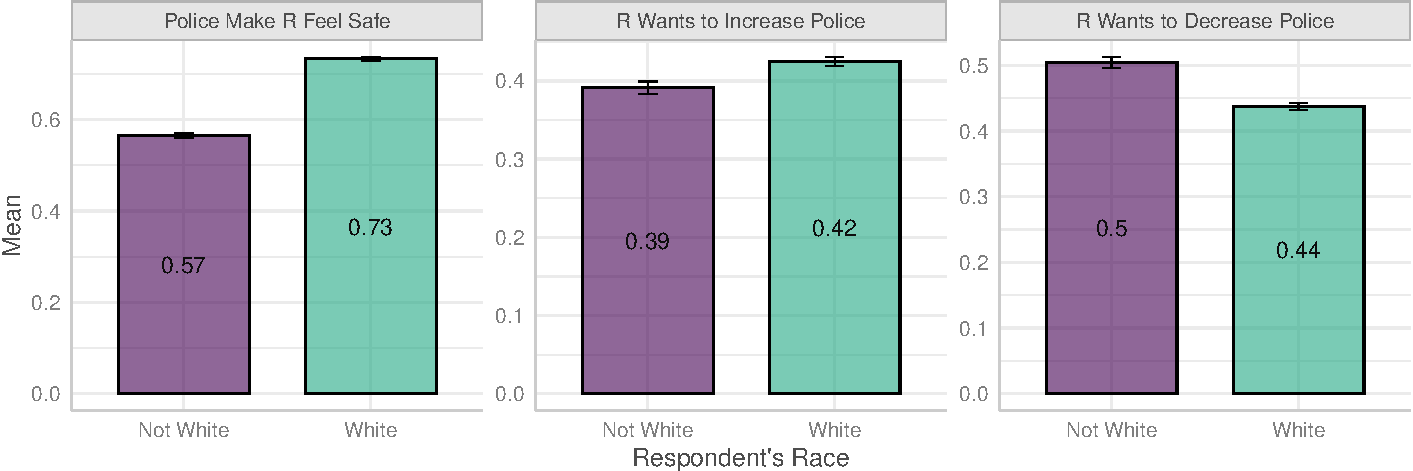
\includegraphics{racialized-police_files/figure-pdf/fig-attitudes-1.pdf}

}

\caption{\label{fig-attitudes}\textbf{Attitudes toward Police by Race.}
All respondents in 2020 CES. Black error bars at the top of columns
indicate the 95\% confidence interval of the estimated attitude. Within
each attitudinal outcome, the difference between non-Hispanic whites and
other respondents is significant at the level of 0.05.}

\end{figure}

On a binary scale of yes or no, the 2020 CES asks the respondents
whether the presence of police makes them feel safe (``police felt as
safe''), whether they support increasing police funding at the expense
of sacrificing some budget for other public services (``increase
police''), and whether they are for decreasing police funding to better
support other public programs (``decrease police''). While the first
question tries to directly measure one's given perception of local
police, the latter two capture the respondent's attitudes on how police
should be maintained or regulated. To ease our interpretation of later
analyses, I linearly coerced the original responses so that for each
question, 1 indicates an affirmative response and 0 a negative one.

Figure~\ref{fig-attitudes} shows descriptive statistics of attitudes
toward police by racial groups. A clear racial divide stands out:
Compared to people of color, non-Hispanic white respondents in 2020 CES
are more likely to feel police as an addition to their safety, more
likely to support increasing the presence of police, and less likely to
endorse reducing the number of police officers. Consistent with our
perception in the real world, such differences on police attitudes are
all significant at the level of 0.05.

\hypertarget{racial-imagery-of-local-police}{%
\subsection{Racial Imagery of Local
Police}\label{racial-imagery-of-local-police}}

By the time when this study was conducted, there is no data source that
captures the universe of racial compositions of all police agencies in
the United States. To measure representation of different racial groups
in local police agencies, this study needs the racial breakdown of
police officers of a given police agency on the one hand, and racial
structure of the locality it serves on the other. For the first
requirement, I choose the 2016 Law Enforcement Management and
Administrative Statistics (LEMAS) that were collected by the Bureau of
Justice Statistics under the U.S. Department of Justice. Started in
1987, LEMAS periodically collects data from more than 3000 state and
local law enforcement agencies, including all those that employ over 100
sworn officers as well as a nationally representative sample of smaller
police agencies. Among the agency-level characteristics surveyed by
LEMAS are the demographic structure of their employees, the place they
serve, and their address in terms of zip code.
Figure~\ref{fig-lemas-cover} shows the county-level coverage of 2016
LEMAS sampling, where counties are colored blue if at least one police
department within its jurisdiction is surveyed. Though apparently having
sampled more police departments in more populated areas, the 2016 LEMAS
in general has a geographically comprehensive coverage. Since most
municipalities in the United States are served by only one police
agency, it is reasonable to infer the police's racial imagery of a place
by looking at the racial compositions of its local police employment. I
extract from the 2016 LEMAS data the total number of sworn officers in a
police agency and the respective numbers of white, Hispanic, and Black
officers, and then calculates the share of each racial group in the
agency' employment.

\begin{figure}[tb]

{\centering 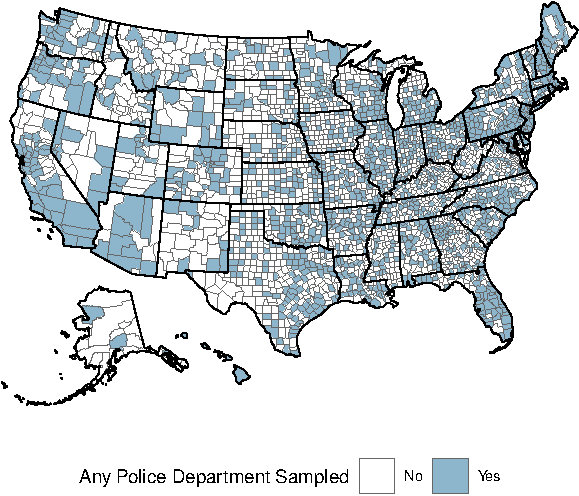
\includegraphics{racialized-police_files/figure-pdf/fig-lemas-cover-1.pdf}

}

\caption{\label{fig-lemas-cover}\textbf{Geographic Coverage of 2016
LEMAS at the County Level.} Counties are colored blue where at least one
police department within its jurisdiction is surveyed in 2016 LEMAS.}

\end{figure}

Given that the share of a racial group in police employment is a general
reflection of its percentage in local population, we can hardly
distinguish the effect of demographic structure from that of racial
composition of police officers if simply looking at the absolute value
of racial shares. A more precise approach would be to measure racial
representation in police by measuring the extent to which the presence
of a racial group exceeds or falls short of its presence in the local
population. This study hence measures racial representations in police
using the gap between the shares of a racial group in police workforce
and in the total population of a place. On a positive-negative spectrum,
a large value of this difference for a racial group means that in this
place, a racial group is better represented in a police agency. For
example, if white Americans count for 70 percent of total population of
a city but over 90 percent of the city's police officers are white, then
black representation in police of the city would be 0.20, meaning an
excess of representation for whites in the police workforce and thereby
a ``whiter'' appearance of police officers.

\begin{figure}[tb]

{\centering 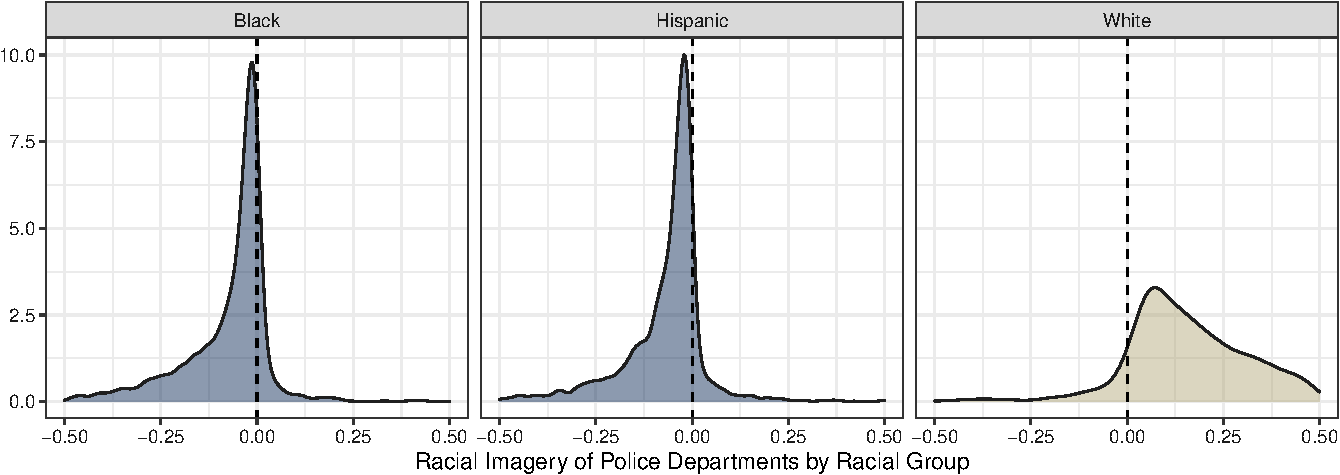
\includegraphics{racialized-police_files/figure-pdf/fig-lemas-density-1.pdf}

}

\caption{\label{fig-lemas-density}\textbf{Distribution of Racial
Presence among Police Departments Surveyed in LEMAS 2016.} Racial
imagery is measured by the difference between a racial group's share in
police officers and in local population. A positive value indicates that
the corresponding racial group is excessively represented in local
police departments, and a negative value the otherwise.}

\end{figure}

Figure~\ref{fig-lemas-density} shows the distribution of racial
representations among the police departments surveyed in 2016 LEMAS. For
most police departments, whites are excessively represented in its
workforce, whose share notably exceeds their percentage in the overall
population. The median level of white representation is greater than 0
and its distribution is apparently right-skewed. For a considerable
number of departments, the level of excessive representation is beyond
0.2, creating a strongly whiter imagery of police officers.
Representations for African and Hispanic Americans, on the other hand,
present a opposite pattern. A dominant number of police departments
employ a smaller share of black or Hispanic police officers than their
presence in the population. The descriptive statistics found in 2016
LEMAS are consistent with the journalist and anecdotal evidence that
police employment is not representative of the population it serves,
forging a white imagery.

\hypertarget{local-police-violence}{%
\subsection{Local Police Violence}\label{local-police-violence}}

There have been no successful efforts by governmental agencies at either
local or federal level to systematically document police-involved
homicides. So existing literature addressing police violence has usually
turned to data voluntarily collected by advocacy groups, the most used
of which is that of Mapping Police Violence project. Drawing data points
from other reliable sources of police-involved shootings and collecting
its unique data through diverse channels including social media, local
newspaper accounts, and police reports, the Mapping Police Violence
project has by far the most detailed and accurate record of fatal
shootings by police since 2013.

Mapping Police Violence project reports where every police-involved
fatal shootings took place at zip code level along with what police
agency is responsible for the shooting. This allows this study to
connect CES respondents with their local context of police violence
using zip code and police agency information. To capture the occurrence
of police violence that are most immediate to a respondent's memory, I
focus on the those police-involved fatal shootings that took place in
2020 before September 29th, the date of the first surveying of 2020 CES.
The vast majority of the places where police violence happened saw only
one incident of such during the range of my observation, and outliners
with more than two police-involved homicides are rare, counting for less
than one percent of all observations. For this reason, I measure the
level of police violence on a binary basis, with 1 that there is at
least one case of police violence recorded in a place.

\hypertarget{results}{%
\section{Results}\label{results}}

\hypertarget{white-attitudes-on-policing}{%
\subsection{White Attitudes on
Policing}\label{white-attitudes-on-policing}}

We first examine the Perception Hypothesis, that is, more representation
of whites in local police workforce should lead to more favorable
perceptions of police among white residents. Figure~\ref{fig-baseline}
shows the estimates on the relationship between racialized imagery of
police workforce and whites' attitudes on policing. Based on an
individual regression among white respondents of 2020 CES, each point
represents the estimated effect of the related racial imagery (indicated
by the horizontal axis) on one's policing attitudes. As whites' presence
in local police workforce increases relative to its share in local
population, whereby a ``whiter'' imagery of police officers emerges,
white Americans are more likely to claim that police make them feel
safe, and they are less willing to decrease the funding for police to
support other public services. No significant effect of white imagery
was found for the attitude on increasing police funding, but the
positive sign of the point estimate is consistent with our expectation.
In contrast, increased representation of African or Hispanic Americans,
which results in a police team that looks less like white people, is
associated with more negative feelings toward policing among white
Respondents. In either case, whites are less likely to perceive police
as safe or support an increase in police funding, and are more likely to
support decreasing police resources.

\begin{figure}[tb]

{\centering 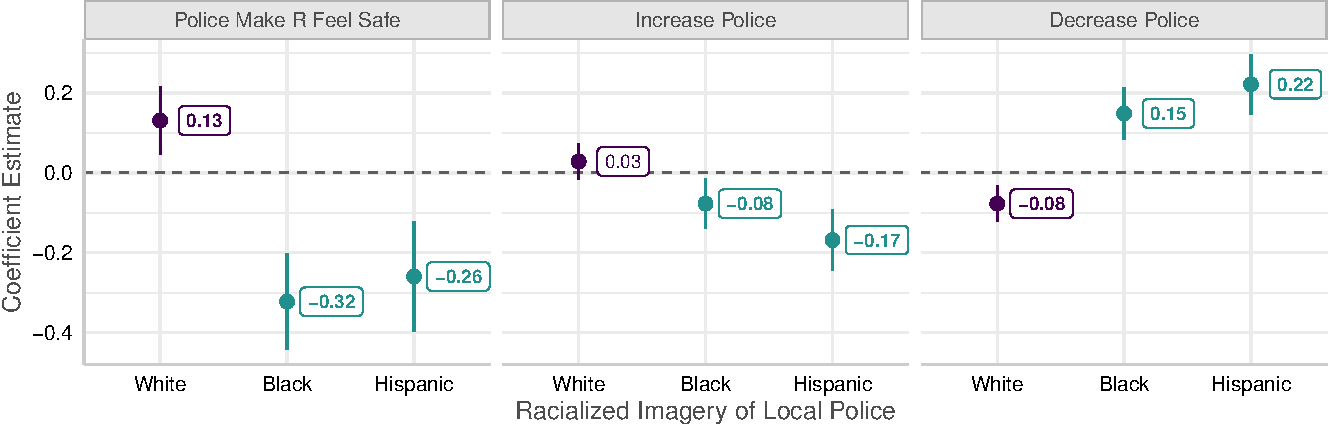
\includegraphics{racialized-police_files/figure-pdf/fig-baseline-1.pdf}

}

\caption{\label{fig-baseline}\textbf{The Estiamted Relationship between
Racial Imagery of Local Police and White Attitudes on Policing.} Each
point indicates the coefficient estimate of the realted racial imagery
on policing attitudes out of an invididual regression among white
respondents in 2020 CES. 95\% confidence intervals are shown by the
range. The strip of each panel indicates the outcome variable of
interest. Positive estimates are colored blue, and significant estimates
(p \textless{} 0.05) are marked in bold text. White percentage in local
population is controlled for.}

\end{figure}

Analyses in Table~\ref{tbl-divides} further looks into the extent to
which overall whiter imagery of police workforce contributes to the
current racial divide on policing attitudes. Here respondents of all
racial identities are included in the regressions. Taking the value of
the respondent's white identity, the term Racial Divide captures the
systemic difference between whites and people of color regarding their
attitudes on policing. Further, the interaction term between racial
divide and police's white imagery, when combined with the standalone
term of racial divide, estimates how racial imagery of police workforce
moderates the racial gap. Results indicate that regardless of the level
of police's white imagery, whites in general are more favorable of
police across the three attitudinal indicators. The racial gap on
feeling police as safe is exacerbated by a whiter imagery of police,
while the gaps on increasing or decreasing police funding are not.

\hypertarget{tbl-divides}{}
\begin{table}
\caption{\label{tbl-divides}Racial Imagery of Local Police Moderates Racial Divides on Policing
Attitudes }\tabularnewline

\centering
\begin{threeparttable}
\begin{tabular}[t]{lccc}
\toprule
  & Police Felt as Safe & Increase Police & Decrease Police\\
\midrule
Racial Divide & 0.389*** & 0.033** & -0.055***\\
 & (0.020) & (0.010) & (0.010)\\
White Imagery of Police & -0.270*** & -0.006 & -0.010\\
 & (0.057) & (0.028) & (0.029)\\
Racial Divide × White Imagery & 0.359*** & 0.020 & -0.041\\
 & (0.070) & (0.035) & (0.036)\\
\midrule
Observations & 39551 & 39597 & 39589\\
R squared & 0.061 & 0.001 & 0.005\\
\bottomrule
\end{tabular}
\begin{tablenotes}
\item Note: All respondents in 2020 CES. The term Racial Divide takes the value of the respondents white identity, 1 if white and 0 if not white, thereby capturing the difference of whites on policing attitudes as compared to people of color. Robust standard errors in parentheses. + p $<$ 0.1, * p $<$ 0.05, ** p $<$ 0.01, *** p $<$ 0.001.
\end{tablenotes}
\end{threeparttable}
\end{table}

But when we are concerned about not the continuous variation of racial
gap but whether there is a gap at all, a different landscape shows up.
Building upon the OLS results in Table~\ref{tbl-divides},
Figure~\ref{fig-divides} presents whether the racial gap on policing
existed as a function of white imagery of police. Ranges where the
effect of white identity is not significantly from 0 at the level of
0.95 are colored red and indicated by blue reference lines. As the white
imagery of local police decreases, we see that the racial gap in feeling
police as safe notably declines and eventually diminished when the
police workforce are least white. For the attitudes on increasing or
decreasing police funding, even though less variation across levels of
racial imagery is found, it is still clear that when whites become
insufficiently represented in police workforce, the racial gap slightly
declines and are eventually not significant. This means that in places
where police officers appear less white, whites and people of color are
generally not so divided or not divided at all with regard to their
perceptions of and visions for policing.

\begin{figure}[tb]

{\centering 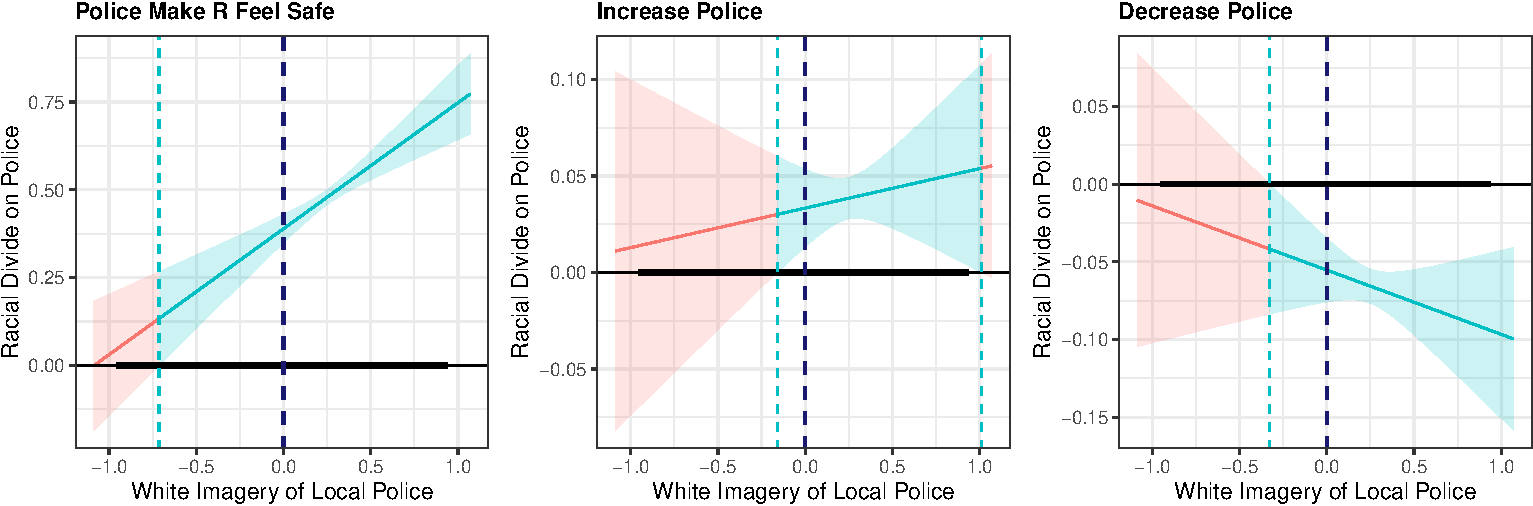
\includegraphics{racialized-police_files/figure-pdf/fig-divides-1.pdf}

}

\caption{\label{fig-divides}\textbf{Racial Imagery of Local Police
Moderates Racial Divide regarding Attitudes on Policing.} Each plot
shows the racial divide on the outcome policing attitude as the white
imagery of local police increases. Ranges of racial imagery where racial
divide diminishes are colored red and indicated by blue reference lines.
The thicker black bar represents the observed range of white imagery of
police in our data.}

\end{figure}

The results from the analyses above build up our confidence that racial
imagery of police workforce, specifically racial compositions of local
police officers relative to the racial structure of local population, is
a shaping force on white people's attitudes on policing. As the police
team gets ``whiter'', whites are more favorable of the role of police.
Racial imagery of police also affects the racial gap on policing
attitudes, places with higher representation of whites in police
employment seeing a larger racial divide. Based on these finding, in the
next part we turn to how racial imagery of police moderates white
people's attitudinal responses in the after of police-involved fatal
shootings.

\hypertarget{white-reaction-to-police-violence}{%
\subsection{White Reaction to Police
Violence}\label{white-reaction-to-police-violence}}

Now we turn to the Defense Hypothesis that expects the occurrence of
police violence will be less effective in persuading whites into more
skeptical attitudes toward police when local police officers present a
stronger white imagery. Table~\ref{tbl-reaction} shows the moderating
effect of racial imagery of police on white people's reaction to local
police violence. Quite intuitively, the occurrence of police violence
during has a negative impact on white's perception of policing, making
them less likely to feel police as safe or support increasing police
funding, and more likely to consider cutting police funding in support
of other public services. But this attitudinal reaction of whites to
police violence is strongly moderated by the racial imagery of local
police, with the interaction term significantly going against the sign
of the main term. As local police present more of a white imagery, the
happening of police violence is less effective in pushing whites toward
more negative views on policing.

Plotting linear predicted values of policing attitudes based on results
in Table~\ref{tbl-reaction}, Figure~\ref{fig-reaction-mod} communicates
this moderating effect of racial imagery of police in more
straightforward way. At each given level of white imagery of police, the
distance between the black point and the green point indicates the
impact of police violence occurrence on white people's policing
attitudes. We can see that across the three outcome variables, the
happening of police violence results in the greatest shift of white
attitudes when whites are insufficiently represented in police workforce
(-0.1). As the representation level of whites in police rises to 0.2,
thereby producing a ``whiter'' imagery of police, the attitudinal shift
is weakened but still existing. When whites are overwhelmingly
over-represented in police, however, almost no difference is observed
between those facing local police violence and those who are not,
indicating a diminishing of the persuasion effect of police violence
occurrence. Overall, greater white presence in police workforce renders
whites of a place more resistant to updating their attitudes on policing
even in the face of the occurrence of police-involved fatal shootings.

\hypertarget{tbl-reaction}{}
\begin{table}
\caption{\label{tbl-reaction}Racial Imagery of Local Police Moderates Racial Reaction to Police
Violence }\tabularnewline

\centering
\begin{threeparttable}
\begin{tabular}[t]{lccc}
\toprule
  & Police Felt as Safe & Increase Police & Decrease Police\\
\midrule
Any Police Violence in 2020 & -0.140*** & -0.057*** & 0.074***\\
 & (0.023) & (0.013) & (0.013)\\
White Imagery of Police & 0.018 & -0.009 & -0.014\\
 & (0.054) & (0.029) & (0.029)\\
Police Violence × White Imagery & 0.260** & 0.078+ & -0.142**\\
 & (0.083) & (0.045) & (0.045)\\
\midrule
Observations & 26016 & 26039 & 26036\\
R squared & 0.004 & 0.002 & 0.003\\
\bottomrule
\end{tabular}
\begin{tablenotes}
\item Note: Non-Hispanic white respondents only, 2020 CES. Robust standard errors in parentheses. + p $<$ 0.1, * p $<$ 0.05, ** p $<$ 0.01, *** p $<$ 0.001.
\end{tablenotes}
\end{threeparttable}
\end{table}

\begin{figure}[tb]

{\centering 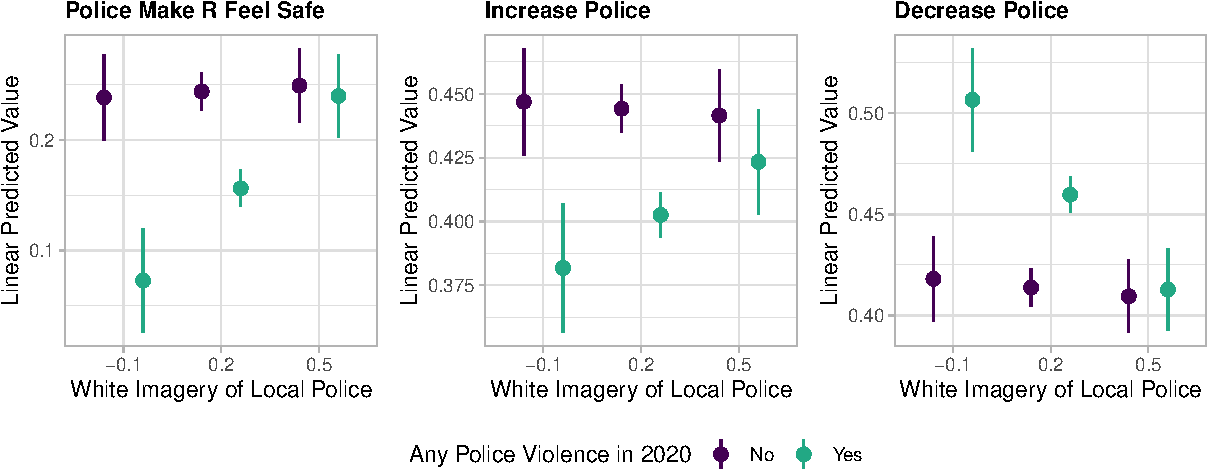
\includegraphics{racialized-police_files/figure-pdf/fig-reaction-mod-1.pdf}

}

\caption{\label{fig-reaction-mod}\textbf{Racial Imagery of Local Police
Moderates Whites' Attitudinal Response to Police Violence.} Based on the
previous OLS analyses with interaction terms, points here represent
linear predicted values of policing attitudes at different levels of
police violence occurrence and racial imagery of local police. At the
each level of racial imagery, whether there police violence happended in
2020 is indicated by the black-green scheme.}

\end{figure}

\hypertarget{examining-the-racial-component}{%
\subsection{Examining the Racial
Component}\label{examining-the-racial-component}}

So far we have observed that as white presence in police workforce
increases, whites will present more favorable views toward policing,
widen their gap on policing attitudes compared to people of color, and
are more resistant to updating their attitudes in the aftermath of
police violence. But how much of this association be attributed to the
racial in-group favoritism fostered among by whites by a ``whiter''
imagery of police officers? This brings us to the empirical test of the
Racialization Hypothesis, which contends that the moderation effect of
police's white imagery on white response to police violence will be
strongest when the cases of such violence are racialized regarding their
victims. Since 2020 CES does not include in its questionnaire in-depth
questions regarding one's racial attitudes or racial consciousness, this
study is unable to directly validate the mechanism. But if it can be
shown that the effect of police's white imagery is strongest in
situations where racial dynamics are emphasized or policing itself is
scrutinized racially, we can have some confidence that racial
consideration is to some extent what drives whites to favor police at
the presence of a ``whiter'' police workforce.

\hypertarget{tbl-racial.component}{}
\begin{table}
\caption{\label{tbl-racial.component}Racial Imagery of Local Police Moderates Whites' Attitudinal Response to
Police Violence }\tabularnewline

\centering
\begin{threeparttable}
\begin{tabular}[t]{lccc}
\toprule
  & Police Felt as Safe & Increase Police & Decrease Police\\
\midrule
PV Whites & -0.129*** & -0.039* & 0.056***\\
 & (0.030) & (0.016) & (0.016)\\
PV POC & -0.152*** & -0.077*** & 0.093***\\
 & (0.029) & (0.016) & (0.016)\\
White Imagery of Police & 0.015 & -0.013 & -0.010\\
 & (0.055) & (0.029) & (0.029)\\
White Imagery × PV Whites & 0.196+ & -0.003 & -0.075\\
 & (0.107) & (0.057) & (0.057)\\
White Imagery × PV POC & 0.327** & 0.162** & -0.210***\\
 & (0.106) & (0.058) & (0.058)\\
\midrule
Observations & 26016 & 26039 & 26036\\
R squared & 0.004 & 0.002 & 0.003\\
\bottomrule
\end{tabular}
\begin{tablenotes}
\item Note: Non-Hispanic white respondents only, 2020 CES. PV Whites means at least one victim of local police violence during 2020 is white. PV POC means that all victims of local police violence during 2020 are people of color. Robust standard errors in parentheses. + p $<$ 0.1, * p $<$ 0.05, ** p $<$ 0.01, *** p $<$ 0.001.
\end{tablenotes}
\end{threeparttable}
\end{table}

Based upon analyses into how racial imagery of police moderates white's
attitudinal response to police violence, this study further separates
the respondents into three categories based on whether police violence
took place in their locality during 2020, and the racial groups impacted
by such police violence. The first group of respondents is those who do
not have police-involved fatal shootings in their place of residence
(``No PV''). The second group live in places where at least one case of
police violence happened, but at least one victim impacted by such
violence is white (``PV Whites''). Similar to the second group, the
third group also sees at least one incident of police violence during
2020, but all racially identifiable victims are people of color (``PV
POC''). Police violence are more likely to activate concerns of racial
justice when predominantly involving people of color. Therefore, though
both affected by police violence, the third group differs from the
second in the sense that racial consciousness may be more prominent to
one's thinking in a more racialized context of police violence. If there
is a racial component in the relationship between police's racial
imagery and white attitudes on policing, we would expect that the
moderation effect of racialized police imagery may be stronger among the
third group than the second.

\begin{figure}[tb]

{\centering 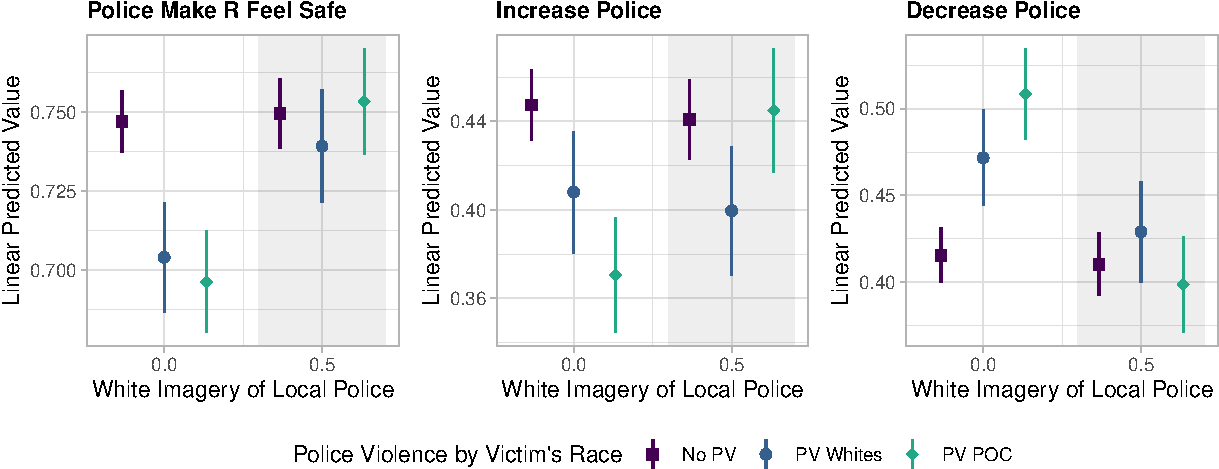
\includegraphics{racialized-police_files/figure-pdf/fig-racial-component-1.pdf}

}

\caption{\label{fig-racial-component}\textbf{Moderating Effect of Racial
Imagery Depends upon Racial Groups Victimized by Police Violence.} Based
on the previous OLS analyses with interaction terms, points here
represent linear predicted values of policing attitudes at different
types of police violence victimization and levels of racial imagery of
local police. At the each level of racial imagery, the racial groups
impacted by local police violence in 2020 are indicated by the
black-to-yellow scheme.}

\end{figure}

Table~\ref{tbl-racial.component} shows the results of our analyses.
Whites' attitudes on policing become less favorable both when police
violence impacts purely people of color and when such violence involves
at least one white victim. But the moderation effect of white imagery of
police is strongest or only present in the case of highly racialized
police violence. For the outcome variable of the respondent feeling
police as safe, whites are less likely to negatively update their views
in the face of police violence if police workforce sees better
representation for whites. This countering effect of racial imagery is
stronger when police violence purely impacts people of color than when
it involves one white victim. For the attitudes on increasing or
decreasing police, however, the moderation effect of police's white
imagery vanishes if at least one white victim is involved in police
violence.

Figure~\ref{fig-racial-component} illustrates more clearly the
heterogeneity of moderation effect of racial imagery contingent upon the
racialization of police violence. Plotting linear predicted values of
policing attitudes based on results in Table~\ref{tbl-racial.component},
Figure~\ref{fig-racial-component} shows at given levels of white imagery
of police, how white attitudes change in response to different types of
police violence, which are indicated by a group of points with different
colors. When white imagery of police violence is low (0), we see that
police violence has great persuasion effect regardless of their victims,
resulting in a notable distance from the baseline points of no police
violence. As white imagery of police violence rises to 0.5, thereby
fostering the perception of police officers as predominantly white, we
see that the attitudinal shit caused by police violence is smaller. When
police violence involves at least one white victim, the shift, though
small, is still observable in terms of point estimates. But when police
violence purely victimizes people of color, we see that the occurrence
of such violence not only fails to shift policing attitudes negatively,
but even pushes the point estimates toward more favorable direction. To
summarize, the fact that the moderation effect of racialized police
imagery is contingent upon the racialization of police violence lends
confidence to our hypothesis that a racial component lies underneath the
association between racial imagery of police and white attitudes on
policing.

\hypertarget{conclusion}{%
\section{Conclusion}\label{conclusion}}

Looking into how racial imagery of local police moderates the way white
respondents perceive police and respond to police violence, this study
offers an identity-oriented approach to disentangling the racial divide
featuring debates on police. This study shows that whites' positive
perceptions of police are associated with better representation of
whites in police workforce that creates a white imagery of the
profession. In places with more of a white imagery in police, a larger
racial divide on policing attitudes emerges. White imagery of police
workforce also repels whites from updating their beliefs about police in
the face of police brutality events, especially when such events are
racialized by the contrast between a white officer and non-white victim.
In a word, racial imagination of police plays a powerful role in shaping
the current racial divide on policing.

Since most data sources that capture detailed feelings and experiences
with police forces fail to disclose residence information of their
respondents, the author is rather constrained to investigate in depth
those psychological processes linking racial representation to one's
perception of local police. Even though the explanation based on racial
imagery is largely self-containing, more specific questions remain
including what factors influence one's processing of such imagery, and
what considerations may outweigh the moderation of racial representation
when one is understanding police violence. Besides, because the number
of Black and Hispanic respondents is too small to generate enough
statistical power after geographic matching in 2020 CES, this study does
not discuss how people of color may also approach police violence
through a lens of racial representation. People of color are in general
better informed about the reality of police brutality, but will they,
like in the case of whites, perceive police more favorably if local
police is more representative of non-whites? Similarly, will people of
color be less triggered by the occurrence of police brutality if the
victim is a white killed by a non-white officer? Empirical examination
of these questions is important, and will be possible in the future with
more detailed and comprehensive data.

This study also generates practical implications for addressing police
brutality in real life. Since people's perceptions of police and police
violence are so strongly conditioned by whether they see local police as
representative of themselves, it would help if we first repair the
representation gap in police employment. This helps foster a non-racial
imagination of police workforce so that people can approach the issue of
police violence through a more pragmatic and less racialized
perspective. Behind the veil of ignorance where police are not perceived
as more of a agent of one race than another
(\protect\hyperlink{ref-rawls1999}{Rawls 1999}), it is more likely that
people with different racial identities can have a meaningful and honest
conversation in full emancipation from racial tribalism.

\section*{Declarations}

\begin{description}
\item[Funding Statement]
This research received no funding.
\item[Conflict of Interest]
The author declares no ethical issues or conflicts of interest in this research.
\item[Ethical Standards]
The author affirms that this research did not involve human subjects. 
\end{description}


\hypertarget{references}{%
\section*{References}\label{references}}
\addcontentsline{toc}{section}{References}

\hypertarget{refs}{}
\begin{CSLReferences}{1}{0}
\leavevmode\vadjust pre{\hypertarget{ref-ahler2018}{}}%
Ahler, Douglas J., and Gaurav Sood. 2018. {``The Parties in Our Heads:
Misperceptions about Party Composition and Their Consequences.''}
\emph{The Journal of Politics} 80(3): 964--981.
\url{https://www.journals.uchicago.edu/doi/10.1086/697253}.

\leavevmode\vadjust pre{\hypertarget{ref-alvarado2020}{}}%
Alvarado, Steven Elías. 2020. {``The Complexities of Race and Place:
Childhood Neighborhood Disadvantage and Adult Incarceration for Whites,
Blacks, and Latinos.''} \emph{Socius: Sociological Research for a
Dynamic World} 6: 1--16.
\url{http://journals.sagepub.com/doi/10.1177/2378023120927154}.

\leavevmode\vadjust pre{\hypertarget{ref-cramer2020}{}}%
Cramer, Katherine. 2020. {``Understanding the Role of Racism in
Contemporary US Public Opinion.''} \emph{Annual Review of Political
Science} 23(1): 153--169.
\url{https://www.annualreviews.org/doi/10.1146/annurev-polisci-060418-042842}.

\leavevmode\vadjust pre{\hypertarget{ref-dawson1995}{}}%
Dawson, Michael C. 1995. \emph{Behind the mule: race and class in
African-American politics}. 1. paperback print. Princeton, NJ: Princeton
Univ. Press.

\leavevmode\vadjust pre{\hypertarget{ref-desilver}{}}%
Desilver, Drew, Michael Lipka, and Dalia Fahmy. 2020. {``10 things we
know about race and policing in the u.s.''}
\url{https://www.pewresearch.org/fact-tank/2020/06/03/10-things-we-know-about-race-and-policing-in-the-u-s/}.

\leavevmode\vadjust pre{\hypertarget{ref-dixon2000}{}}%
Dixon, Travis L., and Daniel Linz. 2000. {``Overrepresentation and
Underrepresentation of African Americans and Latinos as Lawbreakers on
Television News.''} \emph{Journal of Communication} 50(2): 131--154.
\url{https://academic.oup.com/joc/article/50/2/131-154/4110126}.

\leavevmode\vadjust pre{\hypertarget{ref-edsall1992}{}}%
Edsall, Thomas Byrne, and Mary D. Edsall. 1992. \emph{Chain reaction:
the impact of race, rights, and taxes on American politics; with a new
afterword}. 1. publ. New York, NY: Norton.

\leavevmode\vadjust pre{\hypertarget{ref-gay2002}{}}%
Gay, Claudine. 2002. {``Spirals of Trust? The Effect of Descriptive
Representation on the Relationship between Citizens and Their
Government.''} \emph{American Journal of Political Science} 46(4): 717.
\url{https://www.jstor.org/stable/3088429?origin=crossref}.

\leavevmode\vadjust pre{\hypertarget{ref-gilens2009}{}}%
Gilens, Martin. 2009. \emph{Why Americans hate welfare: race, media, and
the politics of antipoverty policy}. Chicago: University of Chicago
Press.

\leavevmode\vadjust pre{\hypertarget{ref-gilliam2000}{}}%
Gilliam, Franklin D., and Shanto Iyengar. 2000. {``Prime suspects: The
influence of local television news on the viewing public.''}
\emph{American Journal of Political Science} 44(3): 560--573.
\url{https://www.jstor.org/stable/2669264?origin=crossref}.

\leavevmode\vadjust pre{\hypertarget{ref-haney-luxf3pez2015}{}}%
Haney-López, Ian. 2015. \emph{Dog whistle politics: how coded racial
appeals have reinvented racism and wrecked the middle class}. Oxford;
New York: Oxford University Press.

\leavevmode\vadjust pre{\hypertarget{ref-hayes2017}{}}%
Hayes, Matthew, and Matthew V. Hibbing. 2017. {``The Symbolic Benefits
of Descriptive and Substantive Representation.''} \emph{Political
Behavior} 39(1): 31--50.
\url{http://link.springer.com/10.1007/s11109-016-9345-9}.

\leavevmode\vadjust pre{\hypertarget{ref-hurwitz2005}{}}%
Hurwitz, Jon, and Mark Peffley. 2005. {``Explaining the Great Racial
Divide: Perceptions of Fairness in the U.S. Criminal Justice System.''}
\emph{The Journal of Politics} 67(3): 762--783.
\url{https://www.journals.uchicago.edu/doi/10.1111/j.1468-2508.2005.00338.x}.

\leavevmode\vadjust pre{\hypertarget{ref-hurwitz1997}{}}%
Hurwitz, Jon, and Mark Peffley. 1997. {``Public perceptions of race and
crime: The role of racial stereotypes.''} \emph{American Journal of
Political Science} 41(2): 375.
\url{https://www.jstor.org/stable/2111769?origin=crossref}.

\leavevmode\vadjust pre{\hypertarget{ref-israel-trummel2022}{}}%
Israel-Trummel, Mackenzie, and Shea Streeter. 2022. {``Police Abuse or
Just Deserts? Deservingness Perceptions and State Violence.''}
\emph{Public Opinion Quarterly} 86(S1): 499--522.
\url{https://academic.oup.com/poq/article/86/S1/499/6604560}.

\leavevmode\vadjust pre{\hypertarget{ref-jefferson2021}{}}%
Jefferson, Hakeem, Fabian G. Neuner, and Josh Pasek. 2021. {``Seeing
Blue in Black and White: Race and Perceptions of Officer-Involved
Shootings.''} \emph{Perspectives on Politics} 19(4): 1165--1183.
\url{https://www.cambridge.org/core/product/identifier/S1537592720003618/type/journal_article}.

\leavevmode\vadjust pre{\hypertarget{ref-jones2016}{}}%
Jones, Philip Edward. 2016. {``Constituents' Responses to Descriptive
and Substantive Representation in Congress*: Constituents' Responses to
Descriptive and Substantive Representation.''} \emph{Social Science
Quarterly} 97(3): 682--698.
\url{https://onlinelibrary.wiley.com/doi/10.1111/ssqu.12243}.

\leavevmode\vadjust pre{\hypertarget{ref-kaslovsky2021}{}}%
Kaslovsky, Jaclyn, Jon C. Rogowski, and Andrew R. Stone. 2021.
{``Descriptive representation and public support for Supreme Court
nominees.''} \emph{Political Science Research and Methods} 9(3):
583--598.
\url{https://www.cambridge.org/core/product/identifier/S2049847019000591/type/journal_article}.

\leavevmode\vadjust pre{\hypertarget{ref-kinder2001}{}}%
Kinder, Donald R., and Nicholas Winter. 2001. {``Exploring the racial
divide: Blacks, whites, and opinion on national policy.''}
\emph{American Journal of Political Science} 45(2): 439.
\url{https://www.jstor.org/stable/2669351?origin=crossref}.

\leavevmode\vadjust pre{\hypertarget{ref-lipsky1980}{}}%
Lipsky, Michael. 1980. \emph{Street-level bureaucracy: dilemmas of the
individual in public services}. New York: Russell Sage Foundation.

\leavevmode\vadjust pre{\hypertarget{ref-mansbridge1999}{}}%
Mansbridge, Jane. 1999. {``Should Blacks Represent Blacks and Women
Represent Women? A Contingent {"}Yes{"}.''} \emph{The Journal of
Politics} 61(3): 628--657.
\url{https://www.journals.uchicago.edu/doi/10.2307/2647821}.

\leavevmode\vadjust pre{\hypertarget{ref-mendelberg2001}{}}%
Mendelberg, Tali. 2001. \emph{The race card: Campaign strategy, implicit
messages, and the norm of equality}. Princeton, N.J: Princeton
University Press.

\leavevmode\vadjust pre{\hypertarget{ref-morin2016}{}}%
Morin, Rich, and Renee Stepler. 2016. {``The racial confidence gap in
police performance.''}
\url{https://www.pewresearch.org/social-trends/2016/09/29/the-racial-confidence-gap-in-police-performance/}.

\leavevmode\vadjust pre{\hypertarget{ref-mutz2015}{}}%
Mutz, Diana Carole. 2015. \emph{In-your-face politics: The consequences
of uncivil media}. Princeton, New Jersey: Princeton University Press.

\leavevmode\vadjust pre{\hypertarget{ref-payne2001}{}}%
Payne, B. Keith. 2001.
{``\href{https://doi.org/10.1037/0022-3514.81.2.181}{Prejudice and
perception: The role of automatic and controlled processes in
misperceiving a weapon}.''} \emph{Journal of Personality and Social
Psychology} 81(2): 181--192.

\leavevmode\vadjust pre{\hypertarget{ref-peffley2010}{}}%
Peffley, Mark, and Jon Hurwitz. 2010. \emph{Justice in america: The
separate realities of blacks and whites}. Cambridge ; New York:
Cambridge University Press.

\leavevmode\vadjust pre{\hypertarget{ref-peffley2007}{}}%
Peffley, Mark, and Jon Hurwitz. 2007. {``Persuasion and Resistance: Race
and the Death Penalty in America.''} \emph{American Journal of Political
Science} 51(4): 996--1012.
\url{https://onlinelibrary.wiley.com/doi/10.1111/j.1540-5907.2007.00293.x}.

\leavevmode\vadjust pre{\hypertarget{ref-phillips2003}{}}%
Phillips, Anne. 2003. \emph{The politics of presence: the political
representation of gender, ethnicity, and race}. Repr. 2003. Oxford:
Oxford Univ. Press.

\leavevmode\vadjust pre{\hypertarget{ref-rawls1999}{}}%
Rawls, John. 1999. \emph{A theory of justice}. Rev. ed. Cambridge, Mass:
Belknap Press of Harvard University Press.

\leavevmode\vadjust pre{\hypertarget{ref-sen2017}{}}%
Sen, Maya. 2017. {``How Political Signals Affect Public Support for
Judicial Nominations: Evidence from a Conjoint Experiment.''}
\emph{Political Research Quarterly} 70(2): 374--393.
\url{http://journals.sagepub.com/doi/10.1177/1065912917695229}.

\leavevmode\vadjust pre{\hypertarget{ref-sen2016}{}}%
Sen, Maya, and Omar Wasow. 2016. {``Race as a Bundle of Sticks: Designs
that Estimate Effects of Seemingly Immutable Characteristics.''}
\emph{Annual Review of Political Science} 19(1): 499--522.
\url{https://www.annualreviews.org/doi/10.1146/annurev-polisci-032015-010015}.

\leavevmode\vadjust pre{\hypertarget{ref-sigelman1997}{}}%
Sigelman, Lee et al. 1997. {``Police Brutality and Public Perceptions of
Racial Discrimination: A Tale of Two Beatings.''} \emph{Political
Research Quarterly} 50(4): 777--791.
\url{http://journals.sagepub.com/doi/10.1177/106591299705000403}.

\leavevmode\vadjust pre{\hypertarget{ref-streeter2019}{}}%
Streeter, Shea. 2019. {``The racial politics of police violence in the
united states.''} PhD thesis.
\url{https://purl.stanford.edu/kf447bj0520}.

\leavevmode\vadjust pre{\hypertarget{ref-tesler2016}{}}%
Tesler, Michael. 2016. \emph{Post-racial or most-racial? Race and
politics in the obama era}. Chicago ; London: University of Chicago
Press.

\leavevmode\vadjust pre{\hypertarget{ref-tesler2012}{}}%
Tesler, Michael. 2012. {``The Spillover of Racialization into Health
Care: How President Obama Polarized Public Opinion by Racial Attitudes
and Race.''} \emph{American Journal of Political Science} 56(3):
690--704.
\url{https://onlinelibrary.wiley.com/doi/10.1111/j.1540-5907.2011.00577.x}.

\leavevmode\vadjust pre{\hypertarget{ref-thomas}{}}%
Thomas, Deja, and Juliana Menasce Horowitz. 2020. {``Support for black
lives matter has decreased since june but remains strong among black
americans.''}
\url{https://www.pewresearch.org/fact-tank/2020/09/16/support-for-black-lives-matter-has-decreased-since-june-but-remains-strong-among-black-americans/}.

\leavevmode\vadjust pre{\hypertarget{ref-valentino2002}{}}%
Valentino, Nicholas A., Vincent L. Hutchings, and Ismail K. White. 2002.
{``Cues that Matter: How Political Ads Prime Racial Attitudes During
Campaigns.''} \emph{American Political Science Review} 96(1): 75--90.
\url{https://www.cambridge.org/core/product/identifier/S0003055402004240/type/journal_article}.

\leavevmode\vadjust pre{\hypertarget{ref-winter2008}{}}%
Winter, Nicholas J. G. 2008. \emph{Dangerous frames: How ideas about
race and gender shape public opinion}. Chicago: University of Chicago
Press.

\end{CSLReferences}



\end{document}
